\documentclass[12pt]{article}

\usepackage{amsfonts,amssymb}
\usepackage[utf8]{inputenc}
\usepackage[russian]{babel}
\usepackage{graphicx}
\usepackage{amsmath}
\usepackage{amsfonts}
\usepackage[ruled, lined]{algorithm2e}
\usepackage{hyperref}

\textheight=220mm
\textwidth=160mm

\newcommand{\sgn}{\operatorname{sgn}}
\newcommand{\argmax}{\operatorname{argmax}}
\newcommand{\NA}{\operatorname{NA}}
\newcommand{\OR}{\operatorname{ or }}
\newcommand{\LCS}{\operatorname{LCS}}
%\DeclareMathOperator{\sgn}{sgn}

\title{\bf Домашнее задание № 2 по курсу \\ <<Параллельные
и распределенные вычисления.>>}
\author{А.Е. Оразаев}
\date{}
\begin{document}

\voffset=-20mm
\hoffset=-12mm
\font\Got=eufm10 scaled\magstep2 \font\Got=eufm10

\maketitle

\section{K-means и openmp.}
\paragraph{Распараллеливание}
В программе сразу можно обратить внимание на большое количество
циклов, которые можно распаралелить:
\begin{itemize}
    \item Первый цикл, который на очередной итерации определяет
          пренадлежность точек кластерам. 
    \item Второй цикл считающий размеры центроидов и вычисляющий
          центроиды для новой итерации.
    \item Третий цикл, вычисляющий новые размеры центроидов.
\end{itemize}

Перед распараллеливанием проведелны следующие рефакторинги:
\begin{itemize}
    \item Перенос расчета размера кластеров в первый цикл.
    \item Уменьшение вложенности второго цикла, который теперь
          занимается только аккумуллированием точек кластеров
          в центроиды.

    \item Уменьшение вложенности третьего цикла и как следствие
          введение еще одного цикла для центроидов, размер которых
          получился равный 0.
\end{itemize}

Далее полученные циклы распаралеливались с помощью средств openmp.

\paragraph{Результаты.}
Замеры времени делались для числа потоков от 1 до 40 по 10 замеров
для каждого потока, далее 40\% замеров для каждого потока отбрасывались
как выбросы и считались средние и минимальные значения.

Данные представляли из себя 50000 точек размерности 700. Эти точки
делились с помощью алгоритма на 50 кластеров.

Результат можно увидеть на графиках:

\begin{center}
    \fbox{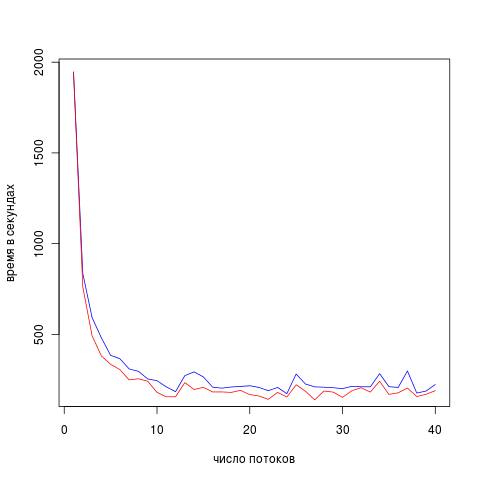
\includegraphics[width=200bp]{hw2.p1/from_1_to_40.png}}
    \fbox{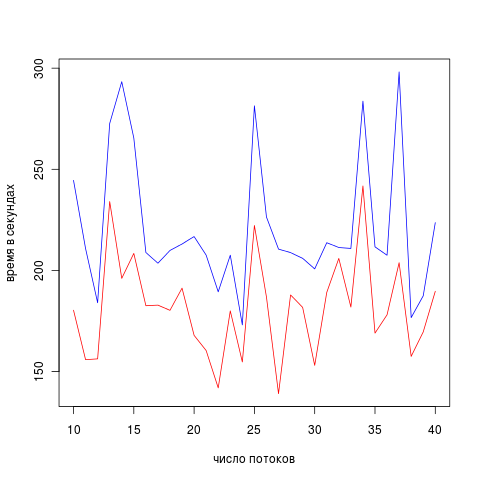
\includegraphics[width=200bp]{hw2.p1/from_10_to_40.png}}
\end{center}

Красной линией отмечены минимальные значения времени, а синей средние.
Можно видеть, что лучшее среднее время программа показывает при использовании
24 потоков, что в принципе ожидаемо, так как задействованы все ресурсы
машины.

\paragraph{Итоги.} Алгоритм был распаралелен, были сделаны практические замеры
времени для различного числа потоков и определено оптимальное число потоков
равное 24, далее можно видеть, что мы фактически не получаем выигрыша во времени.



\section{Игра жизнь.}
\paragraph{Стратегия распараллеливания}
В качестве стратегии распараллеливания была выбрана схема пульсации рассказаная
на лекции. В начале к сетке $ N \times  N $ добавляются лишние ряды для того,
чтобы ряды нацело делились на число потоков выполнения. Далее с помощью
\verb|MPI_Scatter| данные раскатываются по всем потокам. Таким образом
каждый поток владеет несколькими идущими подряд рядами из входных данных.

Возможно и такое, что поток не будет обладать никакими рядами вовсе, то есть
обладать только <<фиктивными>> рядами добавленными в начале. Такое возможно,
если число рядов в матрице соизмеримо с числом потоков, в реальных данных $ N $ 
ожидается многим больше числа потоков, поэтому это потоки с <<фиктивными>> рядами
нам не страшны.

\paragraph{Обмен данными.}
В начале каждой итерации потоки обмениваются верхним и низним рядами со своими
верхним и нижним соседями соответственно. Реализовано это с помощью неблокирующих
функций \verb|MPI_Isend| и \verb|MPI_Irecv|, чтобы во время выполнения передачи
данных потоки могли обработать все остальные ряды, кроме верхнего и нижнего, так
как информации для этого достаточно.

\paragraph{Результаты.}
Замеры производились на случайно сгенерированной сетке $ 5000 \times 5000 $, с
числом итераций равным $ 49 $.

Для каждого числа нод от $ 1 $ до $ 19 $ и для каждого числа процессоров на
от $ 1 $ до $ 12 $ на конкретном числе нод производилось по 10 замеров времени.

Далее как и в прошлой задаче отбрасываись 40\% <<выбросов>> и считалось среднее
и минимальное значение.

Результаты можно увидеть на графиках:
\begin{center}
    \fbox{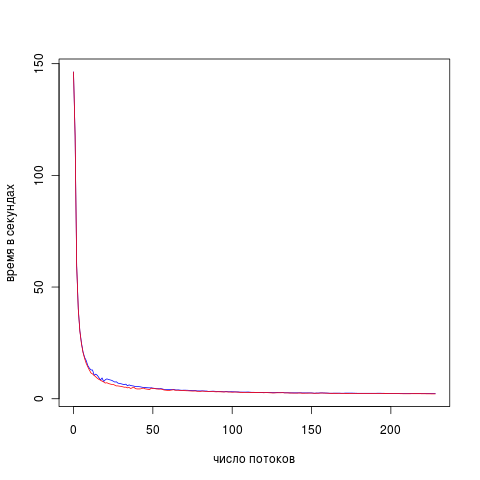
\includegraphics[width=200bp]{hw2.p2/all_values.png}}
    \fbox{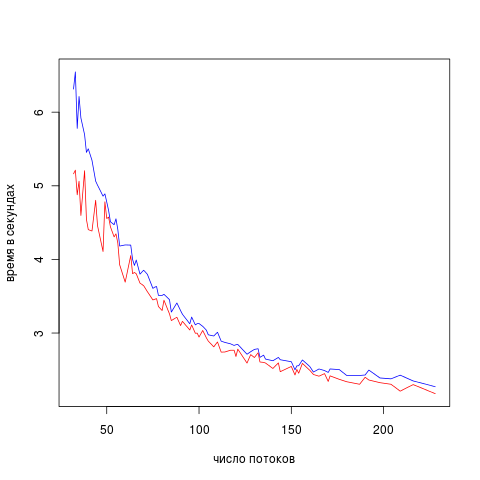
\includegraphics[width=200bp]{hw2.p2/fast_values.png}}
\end{center}
Здесь число потоков -- это число нод умноженное на число процессоров. Красной
линией обозначены минимальные значения, а синей средние.
\begin{center}
    \fbox{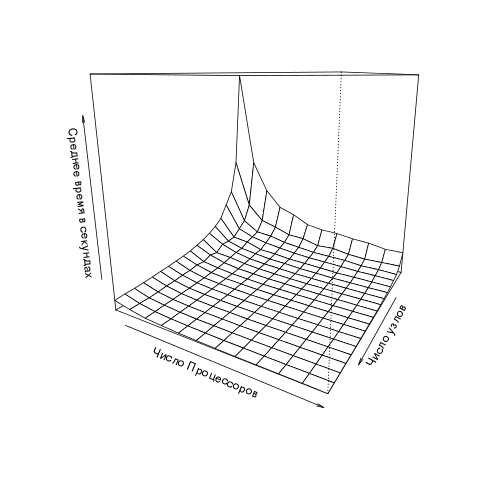
\includegraphics[width=200bp]{hw2.p2/plot_in_3d.png}}
\end{center}
Также следует взглянуть на график зависимости времени не от числа потоков,
а времени от числа процессоров и числа нод, которые фактически и являются
параметрами запуска.

\paragraph{Итоги.} Была написана распределенная версия игры жизнь. Произведены
замеры на различном числе нод и процессоров, в результате определено оптимальное
число потоков -- это $ 228 $, то есть $ 19 $ нод по $ 12 $ процессоров, что в общем
то и очевидно, так как это все ресурсы которые нам даны.

\end{document}
